% GENERATED by experiments/f095_campaign/gen_app_tables.py — do not hand-edit.
\section{f095 Follow-up: Capacity, Symmetry, and Decomposition}
\label{sec:f095}
Unless noted, cells use the same dev E bank ($n_{quartet}{=}237$, $n_{parent}{=}106$), with training seeds 11/23/47; seeds and model arms are not independent datasets. checkpoints, banks, and manifests are in \texttt{artifacts/f095\_campaign/}.
\paragraph{Three-part decomposition.} With per-quartet scores for states A/B/AB, $1-J$ splits into per-case unorderability, no-common-threshold incompatibility, and working-point gap (Fig.~\ref{fig:u03}). Representation (raw$\to$relational) collapses the first segment; flip coverage on relational input collapses the third; incompatibility is the largest segment in every arm.
The split replicates on the order-free D03-E bank ($n{=}1838$ quartets, parents unseen by N models): ordering/incompatibility/working-point segments for raw+flip (0.122/0.648/0.016, 0.179/0.637/0.019, 0.154/0.636/0.053); rel+flip (0.024/0.322/0.051, 0.023/0.275/0.051, 0.020/0.281/0.050) --- same structure as dev512, so the decomposition is not bank-specific.
\begin{figure}[t]
\centering
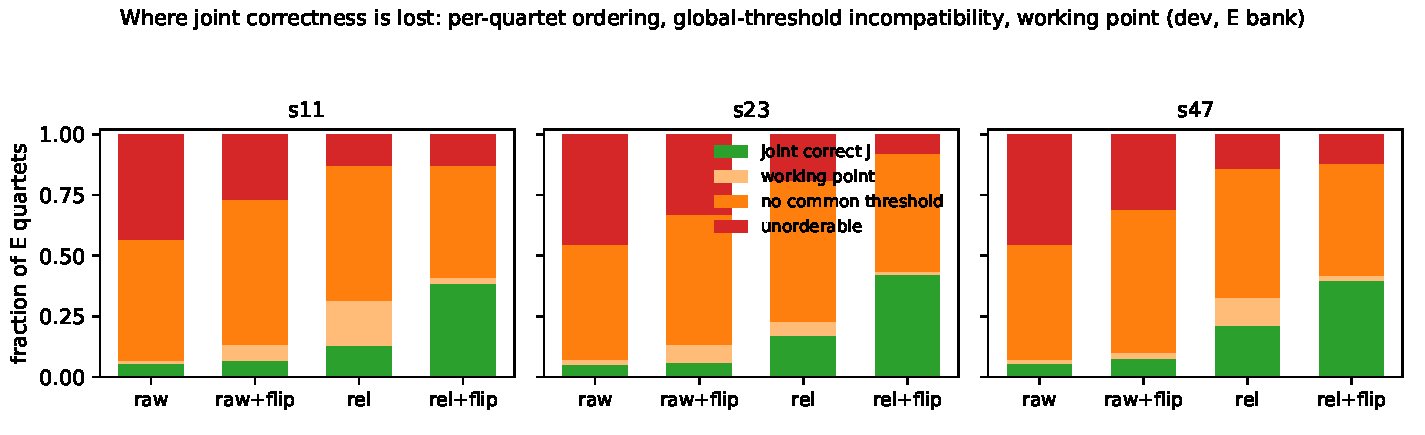
\includegraphics[width=0.95\linewidth]{figures/figU03_decomp.pdf}
\caption{Where joint correctness is lost on the dev E bank (237 quartets, 106 parents): stacked \(1-J\) decomposition per arm and seed. Green is joint-correct J.}
\label{fig:u03}
\end{figure}
\paragraph{Capacity and data frontier (D01, clean arm).} Under the tested recipe, $44\times$ parameters do not improve J; $16\times$ data lifts both arms but does not close the representation gap (Table~\ref{tab:d01}). Flip-BCE runs collapsed in 6/12 cells (flat loss, \(J{=}S{=}0\)); all 6 collapsed cells remain reported; capacity and optimization are not excluded.
\begin{table}[t]
\centering
\small
\begin{tabular}{@{}llll@{}}
\toprule
Cell & params & $J$ (s11/s23/s47) & $S$ \\
\midrule
% w64$\times$N (anchor): .055/.051/.055; w256$\times$N: .025/.046/.038; w512$\times$N: .059/.038/.029; w256$\times$4N: .110/.139/.084; w256$\times$16N: .148/.186/.173
w64$\times$N (anchor) & 6.8k & .055/.051/.055 & .565/.544/.544 \\
w256$\times$N & 84.6k & .025/.046/.038 & .582/.587/.582 \\
w512$\times$N & 300k & .059/.038/.029 & .557/.540/.485 \\
w256$\times$4N & 84.6k & .110/.139/.084 & .688/.709/.722 \\
w256$\times$16N & 84.6k & .148/.186/.173 & .827/.840/.844 \\
\bottomrule
\end{tabular}
\caption{D01 clean-arm frontier. Width cells share train\_101; data cells nest N$\subset$4N$\subset$16N. Full per-seed table with atomic/S/J* in the run JSONs.}
\label{tab:d01}
\end{table}
\paragraph{Symmetry control (D02) and structural follow-ups (U01/U02).} Group-averaging the 8 legal relabelings (same checkpoint, $8\times$ forwards) improves several arms but leaves errors (Table~\ref{tab:d02}); the source-task invariant typed-pair net is worse than raw, while six distances reproduce the relational gain and a depth-matched concatenation does not under this recipe. This does not isolate geometry from optimization.
\begin{table}[t]
\centering
\small
\begin{tabular}{@{}lllll@{}}
\toprule
Arm & $J_{\mathrm{ident}}$ & $J_{\mathrm{avg}}$ & per-\(g\) range & all-8 raw \\
\midrule
raw & .055/.051/.055 & .038/.055/.055 & [0.021,0.110] & .000/.000/.000 \\
raw+flip & .068/.059/.076 & .152/.055/.118 & [0.046,0.114] & .000/.000/.000 \\
rel & .131/.169/.211 & .114/.105/.114 & [0.118,0.211] & .004/.000/.029 \\
rel+flip & .384/.422/.397 & .506/.515/.452 & [0.350,0.494] & .122/.089/.068 \\
typed clean/flip & .013/.025/.008 & .017/.008/.017 & --- & --- \\
sixdist clean/flip & .122/.173/.194 & .439/.426/.253 & --- & --- \\
concat clean/flip & .034/.025/.034 & .059/.084/.046 & --- & --- \\
g8-aug clean/flip & .076/.194/.080 & .363/.308/.245 & --- & --- \\
\bottomrule
\end{tabular}
\caption{Symmetry and structure: group-averaged vs identity J (top, D02); all-8 refers to the original model, not the averaged model. Exact group averaging makes its all-orbit accuracy equal to its identity J. Typed-pair, six-distance, and concatenation follow-ups (middle, U01/U02); symmetry-augmented training (bottom, D02-aug: identity J, disagreement stays .46--.76). s47 sixdist-flip is under-converged (noted, not load-bearing).}
\label{tab:d02}
\end{table}
\paragraph{Coverage response (U07, supported on direction).} 25\%-flip coverage on six-distance exceeds raw at 100\% on both pools (6/6 pool--seed cells; Table~\ref{tab:u07}); on raw, more flip data helps but stays below six at a quarter of the retained flip pool under the tested recipe. Both arms use the same mined pool; this measures retained-example efficiency, not oracle-query savings.
\begin{table}[t]
\centering
\footnotesize
\setlength{\tabcolsep}{3pt}
\begin{tabular}{@{}lllllll@{}}
\toprule
 & N clean & N 25\% & N 100\% & 4N clean & 4N 25\% & 4N 100\% \\
\midrule
raw & .055/.051/.055 & .072/.034/.034 & .068/.059/.076 & .110/.139/.084 & .076/.160/.000 & .228/.279/.236 \\
six & .122/.173/.194 & .270/.321/.350 & .439/.426/.253 & .388/.359/.308 & .443/.460/.439 & .561/.540/.565 \\
\bottomrule
\end{tabular}
\caption{U07 coverage response (dev J). Raw-4N 100\% cells are dedicated flipmine-only reruns: they converge (J .23--.28). Earlier joint-run collapses remain historical outcomes; RNG causation has not been established. Six-25\% exceeds raw-100\% on both pools, 6/6 pool--seed cells.}
\label{tab:u07}
\end{table}
\paragraph{Football geometry (D06, historical single-edit probe).} On 721 real WOY passes, at least one keep and one flip edit within the assumed motion cap exist in 3.0\% at event time (3.2\% successful, 2.5\% unsuccessful) and 3.3\% 1.5\,s before; contested subpopulation (margin$<1$, n=278) 7.2\%. These are single-edit support rates, not E-quartet rates: no A/B/AB joint condition was tested. They do not establish football infeasibility or close natural/partial-observation routes. The zone-crossing anchor is unaffected.
\paragraph{Fresh-bank confirmation (D09, confirmed).} On the archived 236-quartet bank, six-distance beats raw by +0.259/+0.364/+0.195 (flip) and +0.106/+0.072/+0.178 (clean): 6/6 frozen predictions hit. An old integer-ID audit excluded 18 quartets; this namespace-based filter was erroneous. Historically, excluding them (n=218) retained the advantage (gaps +.26/+.37/+.22 flip, +.10/+.07/+.18 clean), but this is not a deduplicated result. D03-E ($n{=}1838$) also reproduces the ordering for N models. Its parents are not fresh for every 4N/16N model. Freshness is checkpoint-specific; these are reanalyses, not new sealed confirmations.
\paragraph{Flip-loss weight (LAM, negative-for-cause).} $\lambda\in\{0.25,0.5,2.0\}$ gives J .042/.080/.089 / .068/.084/.059 / .080/.105/.063, under this limited sweep: this sweep does not identify the cause of large-scale collapse; g8 augmentation recovered 6/6 tested cells.
\paragraph{Vision input-scale$\times$init factorial (D04).} ResNet-18 \citep{he2016deep} on rendered quartets, ImageNet-pretrained \citep{deng2009imagenet} versus random init, joint consistency $J$ (pretrained $|$ random), seeds s803/s805/s806: 64px: .353/.367/.272 $|$ .177/.174/.104; 96px: .517/.501/.547 $|$ .064/.431/.366; 128px: .676/.669/.602 $|$ .040/.563/.450; 224px: .720/.737/.709 $|$ .000/.662/.611; head-only with historical BN adaptation at 224px: .221/.225/.232. All inputs are bilinear resizes of the same 64px image, so larger input adds no observation information. At 224px pretrained-minus-random gains are +72.03/+7.49/+9.87pp (mean +29.80pp, all seeds retained); pretraining equivalence is not established. The s803 random arm collapses at 128/224px, but its cause is unresolved. Historical head-only runs updated BN buffers and were not pure frozen probes. Without a static-only same-architecture arm, these results establish task competence, not a flip-repair effect.
\paragraph{Relation supervision to an image student (U06, historical recipe).} ResNet18 student, same images/labels: endpoint-only (A), +generic-geometry aux (B), +relation aux (C). J: A .353/.367/.272, B .296/.229/.212, C .285/.358/.278; shuffled-target sanity 0.249. At 224px the ordering repeats (A .720/.737/.709; B .691/.506/.713; C .691/.735/.687; shuffled .708/.673/.686): C does not improve A in these runs. Ordered endpoint targets can differ despite identical inputs from the renderer; exact indistinguishability is not assumed for every old-renderer orbit. Shuffled-target and training RNG were not isolated. These observations bound the old recipe and neither prove a noise-regularization mechanism nor rule out relation supervision.
\paragraph{Readout refit (U04, layer complementarity supported, narrowed).} Frozen-encoder refits (linear probes on frozen features \citep{kumar2022finetuning}) yield similar final-score ordering under the tested readouts (relflip static-readout S 0.8734/0.9198/0.8819); flip-readout gains appear on the static relational encoder (relfeat +0.059--0.160); the tested small-MLP adds <+0.021; broader nonlinear readouts remain untested. S is a property of the encoder-head composition, not of the encoder alone; flip readout on raw encoders only migrates errors (R\_full .05--.06, M .39--.48).
\paragraph{Nearest-neighbor comparison (D08, training-path confound).} PCT-style continuation and scratch flipmine attain similar J (+0.008/-0.038/+0.000 on rel); balanced-half and random-half are within range on 2/3 and 1/3 seeds; temperature calibration moves no argmax decisions (24/24 cells), an algebraic identity, not a working-point exclusion. PCT starts from clean weights while flipmine starts from scratch, so this is not a loss-causal comparison. Balanced-half balances flip endpoint classes, not preserve/flip. Training-set regression cannot rule out unseen-parent regression or U05.
\paragraph{Decision policies (D10, historical incomplete enumeration).} For the archived dev-selected policy comparisons, flip-minus-clean is median +0.236/+0.105/+0.085 (historical intervals); these points are not a complete action frontier, and the old isotonic implementation was incorrect. Dev-matched coverage drifts on eval; these values do not establish equal eval coverage or exclude calibration.
\paragraph{Cross-task input advantage (U10).} T1 uses 2,724 E quartets from 322 parents; T2 3,443 from 369. P-A compares inputs under the same flip protocol: distance+flip exceeds raw+flip by +0.500/+0.563/+0.534/+0.392/+0.358/+0.356 (T1 then T2, three seeds each). P-B compares retained flip examples: distance-25\% exceeds raw-100\% in 6/6 cells. Neither test is an interaction test. The original J-scale interaction $I=(J_{distance+flip}-J_{distance})-(J_{raw+flip}-J_{raw})$ is T1 +0.3936/+0.4393/+0.4127; T2 -0.1891/-0.1719/-0.2503. T1 supports positive interaction; T2 is a negative-interaction boundary despite near-perfect combined J. T1 uses six pairwise distances; T2 uses three role-specified distances. The old typed P-C does not establish invariance because indexed normalization breaks exchangeability; corrected retraining is reported below.
Orbit averaging replicates cross-task: it lifts flip-trained arms (T1 six +0.062/+0.041/+0.090; T2 raw +0.069/+0.069/+0.067), 12/12 flip cells positive per task, has small clean-arm effects. Old typed changes below .01 do not demonstrate exact end-to-end invariance; that claim requires corrected preprocessing and retraining.
\paragraph{Collapse recovery (D08-six, cause unresolved).} A preserve-loss (pct) rerun on sixdist rescues the s47 collapse (J 0.376/0.439/0.452 vs flip-BCE .439/.426/.253; pct mean .422 vs flipmine .373). Continuation from clean and scratch training differ, so recovery cannot be attributed to the protection loss alone.
\paragraph{Decision frontier across encoders (D10-ext).} The historical dev-matched policy differences also occur for stronger encoders: rel12 median +0.449/+0.199/+0.217; sixdist median +0.208/+0.118/+0.315; positive-pair fraction .95--1.0 everywhere. These archived points retain the enumeration/calibration limitations above and require corrected policy analysis.
\paragraph{Readout refit on the order-free bank (U04-E).} The scoped P2 pattern replicates on D03-E ($n{=}1838$): flip-readout helps static relfeat encoders (s11 +0.045, 3/3 positive) but not already-flip-trained ones; static-S matches D03 values within .002 (float-level borderline quartets).
\subsection{Corrected pipeline and paired reanalysis}
These are repaired-pipeline runs and reanalyses of exposed banks, not new sealed confirmations. Four-arm intervals resample the same parent groups jointly (2,000 bootstrap draws). Small differences from historical I above arise from recomputing unrounded per-quartet outputs.
\begin{table}[t]\centering\small
\begin{tabular}{@{}llll@{}}\toprule
Task & Seed & $I$ [parent 95\% CI] & corrected typed+flip $J$ \\
\midrule
T1 & 11 & +0.3935 [+0.3410, +0.4453] & 0.2761 \\
T1 & 23 & +0.4394 [+0.3875, +0.4846] & 0.1780 \\
T1 & 47 & +0.4126 [+0.3607, +0.4600] & 0.2684 \\
T2 & 11 & -0.1891 [-0.2444, -0.1305] & 0.3398 \\
T2 & 23 & -0.1719 [-0.2232, -0.1177] & 0.3189 \\
T2 & 47 & -0.2504 [-0.3038, -0.1968] & 0.3404 \\
\bottomrule\end{tabular}
\caption{Corrected U10 analysis. T1: 2,724 quartets/322 parents; T2: 3,443/369. I uses the raw/distance clean/flip arms. Typed models were separately retrained with train-fitted role-shared normalization (18 runs: two tasks, three seeds, clean/25\%/full flip). Typed J remains below distance+flip under this recipe; this is not a parameter- or optimization-matched architecture proof.}\label{tab:u10fixed}\end{table}
\paragraph{Pipeline symmetry.} Saved/reloaded full pipelines give maximum logit differences T1: 21.54$\to$3.05e-05 (prediction differences 0); T2: 23.58$\to$0 (prediction differences 0). T1 residual is float summation tolerance; the old indexed statistics caused substantive differences. Corrected invariance is an engineering result, not an accuracy guarantee.
\paragraph{Visual observability audit.} On 512 training parents, 492/512 have identical images throughout the four within-color endpoint swaps; the other 20 exhibit rasterization differences (maximum pixel difference 0.80). Oracle labels are unchanged throughout. Thus ambiguous identical-image cases exist, but the old renderer is not globally exactly invariant. Orbit target variation cannot be equated with the actual old training loss or its sole failure cause. The repaired renderer sorts same-color endpoints without labels before rendering, yielding identical images for all 512 audited orbits. Subsequent visual comparisons use this changed observation protocol; their old/new absolute J values are not a matched repair effect. The completed canonical visual matrix is reported separately below.
\paragraph{Converged readout reanalysis (O04, partial).} Twelve frozen encoders receive six selected heads each on the exposed dev bank (237 quartets/106 parents). Static-to-flip logistic-head J, averaged over the same three seeds: raw\_clean 0.0563$\to$0.0197; raw\_flipmine 0.0759$\to$0.0816; relfeat 0.1730$\to$0.2644; relflip 0.3404$\to$0.3854. For one identical raw encoder (s11), logistic-flip S=0.5738 but MLP-flip S=0.4810: ordering depends on the head. Head fitting/selection uses parent-separated training subsets, but frozen encoders had seen head-dev parents. All 144 convex candidate fits converged; nonlinear claims remain limited to the tested 16/64-unit heads. This is exposed-bank evidence, not a new-task prospective validation of the decomposition. A prospectively predicted external intervention and downstream echo were not run.
\paragraph{Fair continuation (R07).} Thirty arms (two inputs, three seeds, five methods) run 300 epochs with equal forward counts; continuation methods share each seed's clean weights. On 237 exposed development quartets/106 parents absent from training, mean J for plain/protection is raw 0.0745/0.0689; rel 0.3783/0.3910. Protection-minus-plain signs vary across seeds, so the old loss-causal interpretation is not recovered. Old-correct atomic regression on these unseen parents spans 11.4\%--38.4\% across arms; training-set regression cannot close unseen-atomic protection as a route. This does not constitute a new U07 full-dose matrix or sealed confirmation.
\paragraph{Football E construction (R08/O05).} From 240 sampled events across three existing matches, 670/1449 legal receiver candidates and 48/155 eligible observed selected passes admit an E quartet in the bounded guided/random search. These are searched controlled geometric events, not natural E incidence or counterfactual pass-success labels. The perturbation cap is an empirical displacement envelope, not a joint-dynamics guarantee. An incomplete-player test match required exclusions. Past-only last-position/constant-velocity plus analytic geometry baselines were evaluated under controlled 0.2-second stale inputs; natural-missingness learning and learned partial-observation models were not run. Thus the old infeasibility claim is withdrawn, without promoting this probe to a learned football method.
\paragraph{Repaired policy enumeration (R09).} Three encoders by three seeds are reanalyzed on 43 dev and 96 eval scenes, conditional on oracle feasibility. Candidate score breakpoints and action changes are enumerated with an explicit cost/index tie rule and corrected isotonic regression. The table fixes the dev target coverage at .5 for every pair; actual eval coverage differs, so the quality contrasts are policy extrapolations, not equal-coverage effects.
\begin{table}[t]\centering\small\begin{tabular}{@{}llll@{}}\toprule
Encoder/seed & eval coverage clean/flip & quality clean/flip & paired difference 95\% CI \\
\midrule
raw\_s11 & 0.479/0.323 & 0.391/0.581 & [-0.028, +0.395] \\
raw\_s23 & 0.458/0.406 & 0.364/0.487 & [-0.060, +0.300] \\
raw\_s47 & 0.490/0.490 & 0.319/0.319 & [-0.199, +0.207] \\
rel12\_s11 & 0.448/0.417 & 0.791/0.925 & [+0.012, +0.271] \\
rel12\_s23 & 0.396/0.385 & 0.816/0.946 & [+0.036, +0.247] \\
rel12\_s47 & 0.396/0.323 & 0.921/0.903 & [-0.130, +0.093] \\
sixdist\_s11 & 0.365/0.406 & 0.886/0.923 & [-0.048, +0.133] \\
sixdist\_s23 & 0.344/0.396 & 0.849/0.921 & [-0.062, +0.207] \\
sixdist\_s47 & 0.406/0.396 & 0.923/0.921 & [-0.121, +0.125] \\
\bottomrule\end{tabular}\caption{Repaired dev-selected policy extrapolation on 96 eval scenes. Intervals resample the same scenes and recompute both ratios. Seeds and thresholds are not independent data replications; net utility uses an illustrative reward/cost scale.}\end{table}
\paragraph{Coordinate lineage correction (R03).} Coordinate-level matching reverses the old D09 integer-ID deduction: all 236 D09 quartets have parents absent from N. The historical n218 filter used a wrong namespace; it is not a deduplicated analysis. Seen-parent/new-edit versus unseen-parent counts are:
\begin{table}[t]\centering\small\begin{tabular}{@{}lll@{}}\toprule
Bank & training parents & seen/new-parent quartets \\
\midrule
d03E & 512 & 0/1838 \\
d03E & 2048 & 391/1447 \\
d03E & 8192 & 1838/0 \\
d09fresh665 & 512 & 0/236 \\
d09fresh665 & 2048 & 58/178 \\
d09fresh665 & 8192 & 236/0 \\
dev512 & 512 & 0/237 \\
dev512 & 2048 & 0/237 \\
dev512 & 8192 & 0/237 \\
\bottomrule\end{tabular}\caption{R03 coordinate lineage across 96 checkpoints and three banks. 81 checkpoint training manifests were hash-verified; 15 source-N paths rely on training history. Exact matching against every augmented state was not run. Repeated checkpoint rows are not independent observations.}\end{table}
\paragraph{Matched optimization and retained examples (O01).} 108 scratch candidates cover N/4N, raw/six-distance, 0/25/100\% retained flips, three seeds, and three Adam learning rates (.01/.003/.001), each for 300 steps. Selection uses disjoint static/single dev BCE, never E-J. The new evaluation pool contains 1,229 quartets from 250 eligible parents among 512 sampled parents; 256 separate parents serve development. All failed and successful recipes remain archived.
\begin{table}[t]\centering\small\begin{tabular}{@{}llllllll@{}}\toprule
Size & seed & raw0 & raw25 & raw100 & dist0 & dist25 & dist100 \\
\midrule
N & 11 & 0.0814 & 0.1391 & 0.1440 & 0.2685 & 0.6827 & 0.6428 \\
N & 23 & 0.0732 & 0.1131 & 0.1717 & 0.2766 & 0.6168 & 0.6469 \\
N & 47 & 0.0716 & 0.1310 & 0.1180 & 0.2856 & 0.5899 & 0.6143 \\
4N & 11 & 0.1513 & 0.2685 & 0.4752 & 0.5427 & 0.7681 & 0.8885 \\
4N & 23 & 0.1269 & 0.2620 & 0.3336 & 0.5460 & 0.8145 & 0.8511 \\
4N & 47 & 0.1416 & 0.2685 & 0.4304 & 0.4841 & 0.8096 & 0.8186 \\
\bottomrule\end{tabular}\caption{O01 J under an equal finite optimizer-search budget, on the same 1,229 quartets/250 parents. Distance25 exceeds raw100 in all six size--seed cells. These are retained-label comparisons after mining the full pool, not query savings. Training size is not an independent dataset replication; input dimensions slightly change parameter count.}\end{table}
\paragraph{Confidence timing and orbit metrics (R04/D02).} D03 retention now uses original parent start logits at the train-fixed threshold, with unconditional endpoint and start-correct update denominators separately reported for 72 model/seed/order/edit cells. Actual coverage is reported rather than assumed. This local correction does not alter the original P1B confidence analysis. The repaired D02 audit composes all eight relabelings, verifies averaged logits within float64 tolerance and confirms that averaged-model all8 equals its identity J at an eightfold forward cost. Original-model all8 remains a separate statistic.
\paragraph{Cross-bank dependence.} The old D03 builder also excluded D09 parent IDs in the wrong namespace. Coordinate matching identifies 8 shared E parents, contributing 74 D03 quartets and 14 D09 quartets. These exposed banks are therefore not independent confirmations, even when a model has not trained on their parents. The future builder uses the corrected source offset and asserts the source array; this does not retroactively make the old banks disjoint.
\paragraph{Bounded sampling-access diagnostic (N02, mechanism unresolved).} Twelve frozen checkpoints (three seeds, pretrained/random, trained at 64/224) are evaluated without retraining on the same 64 old-bank quartets from 58 parents. The subset was selected independently of model outcomes with a no-foreground-clipping condition. Each original 64px image is also bilinearly upsampled to 224; four one-pixel translation phases give 24,576 image forwards. At unshifted phase, the input-size swap gives:
\begin{table}[t]\centering\small\begin{tabular}{@{}lllll@{}}\toprule
Seed & checkpoint & $J_{64}$ & $J_{224}$ & parent-mean difference [95\% CI] \\
\midrule
803 & train64\_pretrained & 0.2188 & 0.0000 & -0.2155 [-0.3190, -0.1207] \\
803 & train64\_random & 0.0938 & 0.0000 & -0.0862 [-0.1554, -0.0259] \\
803 & train224\_pretrained & 0.0156 & 0.7031 & +0.6638 [+0.5431, +0.7759] \\
803 & train224\_random & 0.0000 & 0.0000 & +0.0000 [+0.0000, +0.0000] \\
805 & train64\_pretrained & 0.2969 & 0.0000 & -0.3017 [-0.4224, -0.1897] \\
805 & train64\_random & 0.1406 & 0.0000 & -0.1293 [-0.2155, -0.0517] \\
805 & train224\_pretrained & 0.0625 & 0.6719 & +0.5862 [+0.4655, +0.7069] \\
805 & train224\_random & 0.0469 & 0.6250 & +0.5690 [+0.4483, +0.6983] \\
806 & train64\_pretrained & 0.2031 & 0.0000 & -0.2069 [-0.3103, -0.1034] \\
806 & train64\_random & 0.0781 & 0.0000 & -0.0862 [-0.1552, -0.0172] \\
806 & train224\_pretrained & 0.0312 & 0.6875 & +0.6379 [+0.5172, +0.7586] \\
806 & train224\_random & 0.0156 & 0.5625 & +0.5345 [+0.4138, +0.6638] \\
\bottomrule\end{tabular}\caption{N02 frozen-checkpoint input swap; 64 quartets/58 parents shared across all 12 checkpoints. J is quartet-weighted; differences and 4,000-draw bootstrap intervals weight parents equally. Intervals are checkpoint-conditional and not multiplicity-adjusted. The collapsed random seed803 stays in the table.}\end{table}
All six 64-trained checkpoints have zero J after the direct 224 input swap. Thus training at the larger input size cannot be replaced by simply enlarging inputs at inference. Phase sensitivity does not identify aliasing or early downsampling as the cause. Native224/low-pass observation controls, low-stride intervention, full retraining and new-parent prospective confirmation were not run. No sampling mechanism or ImageNet-prior exclusion is established.
\subsection{Completed visual static/flip and observability comparisons}
The canonical within-color endpoint renderer is used for all 21 runs (seven arms, seeds 803/805/806, ResNet-18 at 224 input, 20 training epochs). Evaluation uses the same 159 quartets from 74 physical parents; epochs are selected only by single-dev BCE. Static and flip each expose 2,816 images and take 88 optimizer steps per epoch (1,760 total); static repeats clean images, so parent-level exposure distributions differ. Auxiliary arms share exact image/parent/batch exposure. This changed rendering/data protocol is compared internally, not against old D04 J as a matched before/after effect.
\begin{table}[t]\centering\small\begin{tabular}{@{}lll@{}}\toprule
Arm & $J$ (803/805/806) & mean $J$ \\
\midrule
pretrained\_static & 0.5157/0.6038/0.4969 & 0.5388 \\
pretrained\_flip & 0.6415/0.6981/0.7107 & 0.6834 \\
random\_static & 0.4277/0.4843/0.4843 & 0.4654 \\
random\_flip & 0.7044/0.6541/0.6478 & 0.6688 \\
ordered & 0.7170/0.6415/0.7296 & 0.6960 \\
matched & 0.6981/0.6730/0.7044 & 0.6918 \\
shuffled\_matched & 0.5660/0.7044/0.7421 & 0.6709 \\
\bottomrule\end{tabular}\caption{O03/N01 canonical-renderer comparison on 159 quartets/74 parents. Static/flip rows compare training regimens. Auxiliary rows share the flip-image training exposure; ordered/matched/shuffled use the same initial train-gradient-calibrated weight within a seed. No test J selects epochs.}\end{table}
\begin{table}[t]\centering\small\begin{tabular}{@{}llll@{}}\toprule
Initialization/seed & $\Delta J$ [parent 95\% CI] & 110: full/migration/$n$ & 111 lost/$n$ \\
\midrule
pretrained/803 & +0.1258 [+0.0382,+0.2177] & 20/8/43 & 8/82 \\
pretrained/805 & +0.0943 [+0.0258,+0.1706] & 19/4/34 & 6/96 \\
pretrained/806 & +0.2138 [+0.1152,+0.3176] & 28/4/44 & 7/79 \\
random/803 & +0.2767 [+0.1742,+0.3818] & 34/6/51 & 5/68 \\
random/805 & +0.1698 [+0.0592,+0.2781] & 23/2/34 & 11/77 \\
random/806 & +0.1635 [+0.0625,+0.2722] & 21/1/34 & 12/77 \\
\bottomrule\end{tabular}\caption{Static-to-flip regimen comparison. Parent-paired intervals are positive for all six initialization/seed cells. Full repair and migration share each static model's fixed 110 denominator; old 111 regression uses a distinct denominator.}\end{table}
Mean static-to-flip J increases are 14.47pp pretrained and 20.34pp random. Full repairs exceed migrations within the fixed baseline-110 subsets in all six cells, but some baseline-111 successes regress; neither endpoint accuracy nor aggregate J captures both movements.
\paragraph{Matched targets learn geometry but do not establish extra repair.} For matched versus ordered auxiliary targets, mean J difference is -0.42pp; matched versus BCE-only and shuffled-matched differences are +0.84pp and +2.10pp. Signs are not consistent across seeds; each matched-versus-ordered and matched-versus-BCE J interval crosses zero. Selected-checkpoint normalized matched dev MSE (707 samples/128 parents) is ordered 0.3127/0.4450/0.3191; matched 0.1179/0.2973/0.1853; shuffled\_matched 0.7187/0.7381/0.7932. Matching improves auxiliary learnability, but this protocol does not show it is sufficient for additional joint repair. All three matched-minus-ordered auxiliary-error intervals across 128 dev parents are below zero; this is learnability evidence, not exact geometry recovery. It also does not rule out relation supervision generally. The decision-bottleneck follow-up is running separately; no N03 result is inferred from this gate.
\paragraph{Classical pixel baseline.} Known red/blue color segmentation, PCA line fitting and fixed-stroke endpoint correction feed the analytic crossing rule, without true coordinates or label tuning. Joint correctness is 114/159 (0.717), with atomic joint correctness 128/159 and conditional joint success 114/128. All 2 failed fits among 636 state images remain in the denominator with a fixed negative prediction. Neural superiority is not established; the separate N03 bottleneck experiment must retain this baseline.
